\documentclass[conference]{IEEEtran}
\IEEEoverridecommandlockouts
% The preceding line is only needed to identify funding in the first footnote. If that is unneeded, please comment it out.
\usepackage[german]{babel}
\usepackage{amsmath,amssymb,amsfonts}
\usepackage[backend=biber,style=numeric,sorting=ynt]{biblatex}
\addbibresource{library.bib}
\usepackage{algorithmic}
\usepackage{graphicx}
\usepackage{tikz}
\usepackage{pgfplots}
\usepackage{textcomp}
\usepackage{pdfpages}
\usepackage[utf8]{inputenc}
\def\BibTeX{{\rm B\kern-.05em{\sc i\kern-.025em b}\kern-.08em
    T\kern-.1667em\lower.7ex\hbox{E}\kern-.125emX}}
\usepackage{geometry}
\geometry{
  left=1.5cm,
  right=1.5cm,
  top=1.486cm,
  bottom=2cm
}

\begin{document}

\title{Maschinelles Lernen in der Diagnostik einer Autismus-Spektrum-Störung bei Erwachsenen}

\author{\IEEEauthorblockN{Andreas Zinkl}
\IEEEauthorblockA{OTH Regensburg\\
Regensburg, Deutschland \\
andreas.zinkl@st.oth-regensburg.de}}

\maketitle

\begin{abstract}
In dieser Arbeit wird der Einsatz von Algorithmen aus dem Bereich des maschinellen Lernens für eine hinweisende Diagnose einer Autismus-Spektrum-Störung bei Erwachsenen untersucht. Die in dieser Arbeit verwendeten Open Source Daten enthalten dabei Antworten aus durchgeführten Interviews, basierend auf den DSM\footnote{\label{foot:1}Abkürzung für \glqq Diagnostic and Statistical Manual of Mental Disorders\grqq{}.}-5 Diagnosekriterien. Neben diesen Antworten enthält der Datensatz weitere individuelle Informationen zu den befragten Personen. Im Rahmen der Arbeit werden dabei mit fast allen Algorithmen sehr gute Resultate für eine hinreichende Diagnose mit einer Genauigkeit von bis zu ca. 99\% erreicht.
\end{abstract}

\begin{IEEEkeywords}
Maschinelles Lernen, Autismus, Autismus-Spektrum-Störung, Diagnose, DSM-5
\end{IEEEkeywords}
%%%% CHAPTERS START

\section{Einführung}
Die Zahl der Diagnosen von Autismus-Spektrum-Störungen (ASS) steigt nach \textsc{Weintraub} \cite{Weintraub2011} jährlich stetig an. Diese Diagnosen basieren dabei auf Diagnosekriterien aus einem Katalog von Verhaltens- und Interessensmustern \cite{Weintraub2011, Thabtah2017, Thabtah2018, VanElst2014}. Bei der Diagnose einer ASS werden statistische Diagnosekriterien, basierend auf dem DSM$^{\ref{foot:1}}$-IV, DSM$^{\ref{foot:1}}$-5 und ICD\footnote{\label{foot:2}Abkürzung für \glqq International Statistical Classification of Diseases and Related Health Problems\grqq{}.}-10, zur Detektion verwendet \cite{Thabtah2017, VanElst2014}. Die Bewertung dieser Diagnosekriterien unterliegt dabei dem behandelnden Facharzt und hängt somit auch von dessen persönlicher Einschätzung und Erfahrung ab. Der Ablauf einer Diagnose entspricht dabei einer, aus dem Bereich des maschinellen Lernens und der Biometrie bekannten Vorgehensweise zur Klassifikation von Verhaltensmustern und bietet somit eine Möglichkeit zur Anwendung von Algorithmen aus diesem Bereich an.

\section{Problembeschreibung}
Der für dieses Projekt vorliegende Datensatz wurde bereits von \textsc{Thabtah} \cite{Thabtah2017, Thabtah2018} zur Erstellung eines Konzepts für maschinelle Lernverfahren für die Autismus-Diagnostik verwendet.
% Gibt es Möglichkeiten zur Verbesserung der Probleme?
In diesem Projekt sollen nun konkrete Algorithmen, anhand der Erkenntnisse von \textsc{Thabtah}, zur hinweisenden Diagnose einer ASS verglichen werden. %Dabei können die neu gewonnenen Resultate über die Veröffentlichung als Open Source für neue Entwicklungen zur Unterstützung von Ärzten in der Diagnostik einer ASS verwendet werden. 
Der Vergleich der Algorithmen erfolgt dabei über die aus der Biometrie und des maschinellen Lernens bekannten Verfahren zur Analyse von Verhaltensmustern anhand statistischer Verhaltensanalysen.
\section{Datenvorverarbeitung}
Zu Beginn der Vorverarbeitung ist es zunächst notwendig den Informationsgehalt des Open Source Datensatzes zu analysieren. Im Anschluss daran können in der Datenaufbereitung fehlende Werte interpoliert und Ausreißer gefiltert werden.

\subsection{Beschreibung des Datensatzes}
Der in dieser Arbeit verwendete Datensatz wurde von \textsc{Thabtah} \cite{Thabtah2017, Thabtah}, im Zuge seiner Arbeit zur Erstellung eines Konzepts für die Diagnose einer ASS, im Umfang von 704 Testresultaten gesammelt und veröffentlicht. Die Datensammlung basiert dabei auf den von der Organisation \textsc{NICE} \cite{NICE2012} beschriebenen Richtlinien zur Diagnose einer ASS mit Hilfe des AQ\footnote{\label{foot:3}Test zur Berechnung des Autismus-Spektrum-Quotienten.}-10. Eine Beschreibung des Datensatzes liegt der Veröffentlichung bei, enthält jedoch fehlerhafte sowie unzureichende Informationen und Zuordnungen. Hierzu wird im Rahmen dieser Arbeit der veröffentlichte Datensatz ergänzt und in Tabelle \ref{tbl:datensatz} beschrieben.

\begin{table}[htbp]
\caption{Der Aufbau des Open Source Datensatzes}
\begin{tabular}{l p{6cm}}
\textbf{Attribut-Name} & \textbf{Beschreibung}\\ \hline
age & Alter in Jahren\\
gender & Geschlecht männlich / weiblich\\
ethnicity & Ethnische Herkunft der Person\\
jaundice	 & Mit Gelbsucht geboren\\
autism & Autismus-Diagnose innerhalb der Familie\\
relation & Person, die das Testverfahren durchführt\\
country of residence & Land des Wohnsitzes  \\
used app before & Screening-App bereits zuvor benutzt\\
age desc & Gruppierung des Testverfahrens anhand des Alters\\
A1 & Antwort zur Frage 1 (Trifft zu = 1, sonst = 0)\\
A2 & Antwort zur Frage 2 (Trifft zu = 0, sonst = 1)\\
A3 & Antwort zur Frage 3 (Trifft zu = 0, sonst = 1)\\
A4 & Antwort zur Frage 4 (Trifft zu = 0, sonst = 1)\\
A5 & Antwort zur Frage 5 (Trifft zu = 1, sonst = 0)\\
A6 & Antwort zur Frage 6 (Trifft zu = 0, sonst = 1)\\
A7 & Antwort zur Frage 7 (Trifft zu = 1, sonst = 0)\\
A8 & Antwort zur Frage 8 (Trifft zu = 0, sonst = 1)\\
A9 & Antwort zur Frage 9 (Trifft zu = 0, sonst = 1)\\
A10 & Antwort zur Frage 10 (Trifft zu = 1, sonst = 0)\\
result & Anhand der Antworten errechnetes Gesamtresultat\\
classifiedASD & Mögliche diagnostizierte ASS\\
\end{tabular}
\centering
\label{tbl:datensatz}
\end{table}

\subsection{Datenanalyse und -aufbereitung} \label{sec:analysis}
Das Verfahren zur Zuordnung der einzelnen Datensätze zu den Werten in \textit{classifiedASD} wurde nach \textsc{Thabtah} \cite{Thabtah2017} dabei anhand der von \textsc{NICE} \cite{NICE2012} beschriebenen Richtlinien zur ASS-Diagnose durchgeführt. Dies führt zur in Abbildung \ref{fig:result_classification} dargestellten Verteilung der Daten anhand der Spalten \textit{result} und \textit{classifiedASD}. Dabei ist erkennbar, dass eine eindeutige Zuordnung bereits mit Hilfe der Spalte \textit{result} durchführbar ist.

\begin{figure}[h!]
\centering
% This file was created by matplotlib2tikz v0.6.17.
\begin{tikzpicture}[scale=.8,transform shape]

\definecolor{color0}{rgb}{1,0.498039215686275,0.0549019607843137}

\begin{axis}[
ylabel={Werte in Spalte \textit{result}},
xmin=0.5, xmax=2.5,
ymin=-0.5, ymax=10.5,
xtick={1,2},
xticklabels={ASD Classified,No ASD Classified},
tick align=outside,
tick pos=left,
x grid style={white!69.01960784313725!black},
y grid style={white!69.01960784313725!black}
]
\addplot [black, forget plot]
table {%
0.925 7
1.075 7
1.075 9
0.925 9
0.925 7
};
\addplot [black, forget plot]
table {%
1 7
1 7
};
\addplot [black, forget plot]
table {%
1 9
1 10
};
\addplot [black, forget plot]
table {%
0.9625 7
1.0375 7
};
\addplot [black, forget plot]
table {%
0.9625 10
1.0375 10
};
\addplot [black, forget plot]
table {%
1.925 3
2.075 3
2.075 5
1.925 5
1.925 3
};
\addplot [black, forget plot]
table {%
2 3
2 0
};
\addplot [black, forget plot]
table {%
2 5
2 6
};
\addplot [black, forget plot]
table {%
1.9625 0
2.0375 0
};
\addplot [black, forget plot]
table {%
1.9625 6
2.0375 6
};
\addplot [color0, forget plot]
table {%
0.925 8
1.075 8
};
\addplot [color0, forget plot]
table {%
1.925 4
2.075 4
};
\end{axis}

\end{tikzpicture}
\caption{\em Zuordnung der Datensätze in Abhängigkeit der Werte des Attributes \glqq \textit{result}\grqq}
\label{fig:result_classification}
\end{figure}

Im Verlauf der Arbeit werden jedoch auch weitere Merkmale verwendet, um die Klassifikation anhand der abgegebenen Antworten und Verhaltensweisen der Personen zu untersuchen. Um weitere Merkmale verwenden zu können, wird hierzu eine Datenaufbereitung durchgeführt.

% Vorverarbeitung 
%		-> Fehler ausgebessert / gefiltert
%		-> Normalisierung
%		-> usw..
%		-> Reduktion macht hierbei keinen Sinn! Daten sind bereits stark vereinfacht
Innerhalb der Datenaufbereitung werden in der ersten Analyse Ausreißer mit fehlerhaften oder fehlenden Informationen herausgefiltert. Dabei werden aufgrund von fehlenden Informationen bei den Attributen \textit{ethnicity}, \textit{relation} und \textit{age}, 95 Datensätze für die weitere Verarbeitung entfernt.

Für eine eindeutige Klassifikation ist es außerdem notwendig, die in den Attributen \textit{jaundice} und \textit{autism} enthaltenen nominalen Werte entsprechend zu normalisieren. Hierbei werden die bool'schen Werte \glqq yes\grqq{} und \glqq no\grqq{} zu den numerischen Werten $1$ für \glqq yes\grqq{} und $0$ für \glqq no\grqq{} abgeändert. 

Die ordinalen Werte im Attribut \textit{relation} werden mit Hilfe der \glqq 1-aus-n\grqq{} (engl. \glqq one-hot\grqq) Kodierung aufbereitet. Dies bedeutet, dass für jeden Wert des Attributes eine neue Spalte erzeugt wird. Dabei wird der Wert in der zugehörigen Spalte auf $1$ und in allen anderen Spalten des Attributes auf $0$ gesetzt. %Dies ergibt eine Matrix in der einer Person (repräsentiert durch eine Zeile $i$) ein einziger Wert des Attributes durch eine Markierung der Spalte $j$ mit Hilfe der Funktion $f_{\text{relation}}(i,j)=1$ zugewiesen wird.

Abschließend werden die numerischen Werte $x$ eines Attributes $X$ normiert. In der Normierung der Attribute \textit{age} und \textit{result} wird dabei der maximale Wert des Attributes errechnet und der Anteil des aktuellen Wertes an dem maximalen Wert als normierter Wert ermittelt ($f_{\text{Normierung}}(x) = \frac{x}{\max(X)}$). Somit ergibt sich eine Normierung der Werte im Intervall $[0,1]$.


\section{Merkmalsextraktion}
Basierend auf der Beschreibung des Open Source Datensatzes und der erfolgten Datenanalyse können zunächst die in Tabelle \ref{tbl:features} dargestellten Merkmale extrahiert werden. Dabei wird in dieser Arbeit ein Merkmalsvektor $\vec{v}_M$ ermittelt.

\begin{table}
\caption{Index Beschreibung des Merkmalsvektors}
\begin{tabular}{c p{5cm}}
\textbf{Index} & \textbf{Attribut} \\ \hline
0-9 & A1 - A10 (Antworten von Frage 1 bis 10)\\
10 & result\\
11 & age \\
12 & gender\\
13 & jaundice\\
14 & autism\\
15 & relation self\\
16 & relation parent\\
17 & relation healthcare\\
18 & relation relative\\
19 & relation others\\
\end{tabular}
\centering
\label{tbl:features}
\end{table}

Somit ergibt sich aus der Tabelle \ref{tbl:features} ein Merkmalsvektor $\vec{m} = (m_0, ..., m_n)^T$ mit $n = 19$ und insgesamt 20 Merkmalen. Es ist jedoch zu beachten, dass aufgrund der Datenanalyse, das Merkmal \textit{result} die Problemstellung für den Datensatz bereits löst. Aus diesem Grund werden in der Merkmalsextraktion zwei Vektoren generiert. Dies ist der Merkmalsvektor $\vec{m}_{\text{with-result}}$, welcher das Merkmal \textit{result} enthält, sowie ein Merkmalsvektor $\vec{m}_{\text{without-result}}$ der das Merkmal nicht enthält. Dies ermöglicht in der Evaluation einen Vergleich, ob eine Klassifikation ohne das Merkmal \textit{result} mit gleicher Qualität durchgeführt werden kann.

\section{Auswahl der Algorithmen} \label{sec:algorithms}
Die Auswahl geeigneter Algorithmen, fordert zunächst eine Einordnung der Problemstellung. Die Diagnose einer ASS kann dabei nach \textsc{Müller} und \textsc{Guido} \cite[S.~94]{Muller2016} zur Vorhersage einer Klassifikation zugeordnet werden. In dieser Arbeit werden unterschiedliche Algorithmen mit Hilfe von überwachtem und unüberwachtem Lernen \cite[S.~93]{Muller2016} gegenübergestellt. 
Die in dieser Arbeit gegenübergestellten Algorithmen sind der Entscheidungsbaum (engl. \glqq Decision Tree\grqq), die Support-Vector-Machine (SVM), der K-Nearest-Neighbour sowie der K-Means. %Auf die ebenso mögliche Wahl einer Einklassen-Klassifzierung (engl. \glqq One Class Classification\grqq) wird in dieser Arbeit nicht eingegangen, da hierbei in der Klassifizierung Informationen in den Zusammenhängen der Daten verloren gehen.
Zur Evaluation eines jeden Algorithmus dient die Berechnung der Genauigkeit bzw. Trennschärfe (engl. \glqq Accuracy\grqq{} (ACC)).

\begin{equation} \label{math:accuracy}
\text{ACC} = \frac{\#\text{Richtige Diagnosen}}{\#\text{Durchgeführte Diagnosen}}
\end{equation}

Zudem wird zum näheren Vergleich der Genauigkeit in der Diagnose die Rate der richtig diagnostizierten Datensätze (engl. \glqq True Positive Rate\grqq{} (TPR)) und die Rate der fälschlicherweise diagnostizierten Datensätze (engl. \glqq False Positive Rate\grqq{} (FPR)) verwendet.

\begin{equation} \label{math:fpr}
\text{FPR} = \frac{\#\text{Falsche Autismus-Klassifikationen}}{\#\text{Datensätze mit \textit{classifiedASD} = NO}}
\end{equation}

{\setlength{\parindent}{0cm}
\begin{equation} \label{math:tpr}
\text{TPR} = \frac{\#\text{Richtige Autismus-Klassifikationen}}{\#\text{Datensätze mit \textit{classifiedASD} = YES}}
\end{equation}}

Für jeden Algorithmus werden dabei 30\% der aufbereitenden  Daten (182 Datensätze) zum Training und 70\%  der Daten (427 Datensätze) zur Generierung einer aussagekräftigen Statistik zur Evaluation verwendet. Dabei werden jeweils 30\% der positiven ASS-Diagnosen und negativen ASS-Diagnosen für das Training verwendet, um eine gleichmäßige Verteilung innerhalb der Trainingsdaten zu erhalten. Die Aufteilung der Trainings- und Testdaten erfolgt dabei zufällig zur Laufzeit des Algorithmus. Bei der Auswahl der geeigneten Parameter (z.B. die Wahl des Parameter C im Algorithmus der SVM) wird in dieser Arbeit stets mit Hilfe einer Kreuzvalidierung (engl. \glqq Cross-Validation\grqq{}) durchgeführt.


\subsection{Decision Tree} \label{sec:tree}
Von der Problemstellung und der anschließenden Datenanalyse ausgehend, ist der Algorithmus des Entscheidungsbaumes (engl. \glqq Decision Tree\grqq) sehr gut geeignet. Der Grund diesbezüglich liegt im Vorgang der Diagnostik. Hierbei werden die Fragen schrittweise abgearbeitet. Die Resultate der Fragen werden dabei in zwei möglichen Formen \glqq Trifft zu\grqq{} und \glqq Trifft nicht zu\grqq{} bewertet. Diese Art des Vorgehens ähnelt dabei der Funktionsweise des Entscheidungsbaum-Algorithmus. In dieser Arbeit wird hierzu nun der von \textit{sklearn} implementierte Algorithmus verwendet. Um die Trennschärfe noch weiter zu Verbessern wird eine der Parameter der maximalen Tiefe $d$ des Entscheidungsbaumes $T$ definiert. Die maximale Tiefe $d(T)$ wird dabei für $n$ Merkmale auf $d(T) = n-1$ gesetzt. Dies ermöglicht es, dass für jedes Merkmal maximal eine Entscheidung getroffen wird und führt zur gewünschten Verbesserung der Trennschärfe.

Bereits aus der Datenanalyse (siehe Kapitel \ref{sec:analysis}) ist ersichtlich, dass die Zuordnung der Klassen anhand des Merkmals \textit{result} eindeutig durchführbar ist. Dies bestätigt der in Abbildung \ref{fig:tree_graph} dargestellte Aufbau des Entscheidungsbaumes. Dieser wurde dabei mit Hilfe von 20 Trainingsdaten durch das Framework \textit{sklearn} automatisch generiert. Dabei wählt der Algorithmus ebenso das Merkmal \textit{result} als Entscheidungsmerkmal zur Klassifizierung.

\begin{figure}[h!]
\centering
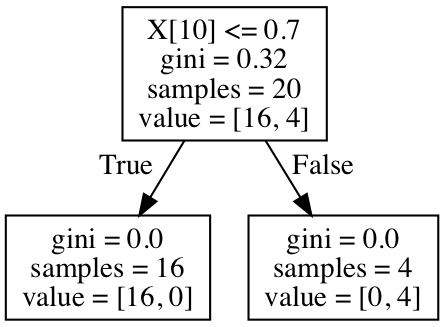
\includegraphics[scale=0.7]{graphs/tree_graph.png}
\caption{\em Automatisierter Aufbau des Decision Tree durch \glqq sklearn\grqq{} durch Prüfung der Merkmale}
\label{fig:tree_graph}
\end{figure} %TODO Hier noch die Parameterwahl der Anzahl an Blätter beschreiben
\subsection{Support-Vector-Machine}
Da es sich bei der Problemstellung um eine Klassifikation von zwei statischen Klassen handelt, ist der Einsatz einer Support-Vector-Machine (SVM) denkbar. Besonders die große Dimension der Merkmalsvektoren ist hierbei ein Grund zur Wahl einer SVM. In dieser Arbeit werden dabei der \glqq Radial Basic Function\grqq{} (RBF) Kernel sowie ein linearer Kernel verwendet.
Die in dieser Arbeit implementierte SVM wird mit Hilfe des Framework \textit{sklearn} umgesetzt. Um eine für die SVM möglichst aussagekräftige Statistik zu erhalten und die bestmöglichen Parameter zu ermitteln, erfolgt bei der Evaluation eine  Kreuzvalidierung. Zudem werden bei der Verwendung der \textit{sklearn}-SVM die Parameter $\gamma$ und $C$ variiert um ein Over- und Underfitting zu vermeiden.

Das Resultat zur Wahl der Parameter zeigt hierbei, dass bei einer Wahl des Paramaters $C=1$ und des zusätzlichen Parameters $\gamma = 0.0977$ für eine SVM mit RBF Kernel, bereits eine Genauigkeit (engl. \glqq Accuracy\grqq{} (ACC)) von ca. 99\% erreicht werden kann (siehe Abbildung \ref{fig:c_chooseSVM} und \ref{fig:gamma_chooseSVM}).

\begin{figure}[h!]
\centering
% This file was created by matplotlib2tikz v0.6.17.
\begin{tikzpicture}[scale=.8,transform shape]

\definecolor{color0}{rgb}{0.886274509803922,0.290196078431373,0.2}
\definecolor{color1}{rgb}{0.203921568627451,0.541176470588235,0.741176470588235}
\definecolor{color2}{rgb}{0.596078431372549,0.556862745098039,0.835294117647059}

\begin{axis}[
xlabel={Parameter C},
ylabel={Accuracy},
xmin=-0.05, xmax=1.05,
ymin=0.688172131147541, ymax=1.00969672131148,
tick align=outside,
tick pos=left,
xmajorgrids,
x grid style={white!80.0!black},
ymajorgrids,
y grid style={white!80.0!black},
axis line style={white!80.0!black},
legend entries={{Linear mit result},{RBF mit result},{Linear ohne result},{RBF ohne result}},
legend cell align={left},
legend style={at={(0.97,0.03)}, anchor=south east, draw=none}
]
\addplot [semithick, color0, mark=*, mark size=3, mark options={solid}]
table {%
1e-100 0.704426229508197
1.02353102189903e-99 0.704426229508197
1.04761575278967e-98 0.704426229508197
1.07226722201033e-97 0.704426229508197
1.09749876549306e-96 0.704426229508197
1.12332403297803e-95 0.704426229508197
1.14975699539774e-94 0.704426229508197
1.176811952435e-93 0.704426229508197
1.20450354025879e-92 0.704426229508197
1.23284673944207e-91 0.704426229508197
1.26185688306603e-90 0.704426229508197
1.29154966501489e-89 0.704426229508197
1.32194114846604e-88 0.704426229508197
1.35304777457982e-87 0.704426229508197
1.38488637139389e-86 0.704426229508197
1.41747416292682e-85 0.704426229508197
1.45082877849595e-84 0.704426229508197
1.48496826225448e-83 0.704426229508197
1.51991108295295e-82 0.704426229508197
1.55567614393049e-81 0.704426229508197
1.59228279334111e-80 0.704426229508197
1.62975083462067e-79 0.704426229508197
1.66810053720008e-78 0.704426229508197
1.70735264747072e-77 0.704426229508197
1.74752840000771e-76 0.704426229508197
1.78864952905746e-75 0.704426229508197
1.8307382802954e-74 0.704426229508197
1.87381742286042e-73 0.704426229508197
1.91791026167252e-72 0.704426229508197
1.96304065004031e-71 0.704426229508197
2.00923300256509e-70 0.704426229508197
2.05651230834869e-69 0.704426229508197
2.10490414451206e-68 0.704426229508197
2.15443469003193e-67 0.704426229508197
2.20513073990309e-66 0.704426229508197
2.25701971963397e-65 0.704426229508197
2.31012970008318e-64 0.704426229508197
2.36448941264543e-63 0.704426229508197
2.4201282647944e-62 0.704426229508197
2.47707635599173e-61 0.704426229508197
2.53536449397014e-60 0.704426229508197
2.59502421139976e-59 0.704426229508197
2.65608778294672e-58 0.704426229508197
2.71858824273297e-57 0.704426229508197
2.78255940220716e-56 0.704426229508197
2.84803586843584e-55 0.704426229508197
2.91505306282522e-54 0.704426229508197
2.98364724028338e-53 0.704426229508197
3.05385550883341e-52 0.704426229508197
3.12571584968823e-51 0.704426229508197
3.19926713779738e-50 0.704426229508197
3.27454916287773e-49 0.704426229508197
3.35160265093885e-48 0.704426229508197
3.43046928631493e-47 0.704426229508197
3.51119173421514e-46 0.704426229508197
3.59381366380464e-45 0.704426229508197
3.67837977182865e-44 0.704426229508197
3.76493580679249e-43 0.704426229508197
3.85352859371055e-42 0.704426229508197
3.94420605943768e-41 0.704426229508197
4.03701725859658e-40 0.704426229508197
4.13201240011537e-39 0.704426229508197
4.22924287438953e-38 0.704426229508197
4.3287612810831e-37 0.704426229508197
4.43062145758392e-36 0.704426229508197
4.53487850812863e-35 0.704426229508197
4.64158883361283e-34 0.704426229508197
4.75081016210285e-33 0.704426229508197
4.86260158006541e-32 0.704426229508197
4.97702356433218e-31 0.704426229508197
5.09413801481645e-30 0.704426229508197
5.21400828799976e-29 0.704426229508197
5.33669923120639e-28 0.704426229508197
5.46227721768442e-27 0.704426229508197
5.59081018251231e-26 0.704426229508197
5.72236765935031e-25 0.704426229508197
5.85702081805677e-24 0.704426229508197
5.99484250318952e-23 0.704426229508197
6.13590727341329e-22 0.704426229508197
6.28029144183437e-21 0.704426229508197
6.42807311728445e-20 0.704426229508197
6.57933224657582e-19 0.704426229508197
6.73415065775097e-18 0.704426229508197
6.89261210434985e-17 0.704426229508197
7.0548023107188e-16 0.704426229508197
7.22080901838563e-15 0.704426229508197
7.39072203352596e-14 0.704426229508197
7.56463327554648e-13 0.704426229508197
7.74263682681147e-12 0.704426229508197
7.92482898353938e-11 0.704426229508197
8.11130830789709e-10 0.704426229508197
8.30217568131997e-09 0.704426229508197
8.49753435908668e-08 0.704426229508197
8.69749002617809e-07 0.704426229508197
8.90215085445065e-06 0.704426229508197
9.11162756115517e-05 0.702786885245902
0.000932603346883218 0.85051912568306
0.00954548456661833 0.916256830601093
0.0977009957299225 0.977021857923497
1 0.995081967213115
};
\addplot [semithick, color1, mark=asterisk*, mark size=3, mark options={solid}]
table {%
1e-100 0.704426229508197
1.02353102189903e-99 0.704426229508197
1.04761575278967e-98 0.704426229508197
1.07226722201033e-97 0.704426229508197
1.09749876549306e-96 0.704426229508197
1.12332403297803e-95 0.704426229508197
1.14975699539774e-94 0.704426229508197
1.176811952435e-93 0.704426229508197
1.20450354025879e-92 0.704426229508197
1.23284673944207e-91 0.704426229508197
1.26185688306603e-90 0.704426229508197
1.29154966501489e-89 0.704426229508197
1.32194114846604e-88 0.704426229508197
1.35304777457982e-87 0.704426229508197
1.38488637139389e-86 0.704426229508197
1.41747416292682e-85 0.704426229508197
1.45082877849595e-84 0.704426229508197
1.48496826225448e-83 0.704426229508197
1.51991108295295e-82 0.704426229508197
1.55567614393049e-81 0.704426229508197
1.59228279334111e-80 0.704426229508197
1.62975083462067e-79 0.704426229508197
1.66810053720008e-78 0.704426229508197
1.70735264747072e-77 0.704426229508197
1.74752840000771e-76 0.704426229508197
1.78864952905746e-75 0.704426229508197
1.8307382802954e-74 0.704426229508197
1.87381742286042e-73 0.704426229508197
1.91791026167252e-72 0.704426229508197
1.96304065004031e-71 0.704426229508197
2.00923300256509e-70 0.704426229508197
2.05651230834869e-69 0.704426229508197
2.10490414451206e-68 0.704426229508197
2.15443469003193e-67 0.704426229508197
2.20513073990309e-66 0.704426229508197
2.25701971963397e-65 0.704426229508197
2.31012970008318e-64 0.704426229508197
2.36448941264543e-63 0.704426229508197
2.4201282647944e-62 0.704426229508197
2.47707635599173e-61 0.704426229508197
2.53536449397014e-60 0.704426229508197
2.59502421139976e-59 0.704426229508197
2.65608778294672e-58 0.704426229508197
2.71858824273297e-57 0.704426229508197
2.78255940220716e-56 0.704426229508197
2.84803586843584e-55 0.704426229508197
2.91505306282522e-54 0.704426229508197
2.98364724028338e-53 0.704426229508197
3.05385550883341e-52 0.704426229508197
3.12571584968823e-51 0.704426229508197
3.19926713779738e-50 0.704426229508197
3.27454916287773e-49 0.704426229508197
3.35160265093885e-48 0.704426229508197
3.43046928631493e-47 0.704426229508197
3.51119173421514e-46 0.704426229508197
3.59381366380464e-45 0.704426229508197
3.67837977182865e-44 0.704426229508197
3.76493580679249e-43 0.704426229508197
3.85352859371055e-42 0.704426229508197
3.94420605943768e-41 0.704426229508197
4.03701725859658e-40 0.704426229508197
4.13201240011537e-39 0.704426229508197
4.22924287438953e-38 0.704426229508197
4.3287612810831e-37 0.704426229508197
4.43062145758392e-36 0.704426229508197
4.53487850812863e-35 0.704426229508197
4.64158883361283e-34 0.704426229508197
4.75081016210285e-33 0.704426229508197
4.86260158006541e-32 0.704426229508197
4.97702356433218e-31 0.704426229508197
5.09413801481645e-30 0.704426229508197
5.21400828799976e-29 0.704426229508197
5.33669923120639e-28 0.704426229508197
5.46227721768442e-27 0.704426229508197
5.59081018251231e-26 0.704426229508197
5.72236765935031e-25 0.704426229508197
5.85702081805677e-24 0.704426229508197
5.99484250318952e-23 0.704426229508197
6.13590727341329e-22 0.704426229508197
6.28029144183437e-21 0.704426229508197
6.42807311728445e-20 0.704426229508197
6.57933224657582e-19 0.704426229508197
6.73415065775097e-18 0.704426229508197
6.89261210434985e-17 0.704426229508197
7.0548023107188e-16 0.704426229508197
7.22080901838563e-15 0.704426229508197
7.39072203352596e-14 0.704426229508197
7.56463327554648e-13 0.704426229508197
7.74263682681147e-12 0.704426229508197
7.92482898353938e-11 0.704426229508197
8.11130830789709e-10 0.704426229508197
8.30217568131997e-09 0.704426229508197
8.49753435908668e-08 0.704426229508197
8.69749002617809e-07 0.704426229508197
8.90215085445065e-06 0.704426229508197
9.11162756115517e-05 0.704426229508197
0.000932603346883218 0.704426229508197
0.00954548456661833 0.704426229508197
0.0977009957299225 0.935983606557377
1 0.981912568306011
};
\addplot [semithick, blue, dash pattern=on 1pt off 3pt on 3pt off 3pt]
table {%
1e-100 0.704426229508197
1.02353102189903e-99 0.704426229508197
1.04761575278967e-98 0.704426229508197
1.07226722201033e-97 0.704426229508197
1.09749876549306e-96 0.704426229508197
1.12332403297803e-95 0.704426229508197
1.14975699539774e-94 0.704426229508197
1.176811952435e-93 0.704426229508197
1.20450354025879e-92 0.704426229508197
1.23284673944207e-91 0.704426229508197
1.26185688306603e-90 0.704426229508197
1.29154966501489e-89 0.704426229508197
1.32194114846604e-88 0.704426229508197
1.35304777457982e-87 0.704426229508197
1.38488637139389e-86 0.704426229508197
1.41747416292682e-85 0.704426229508197
1.45082877849595e-84 0.704426229508197
1.48496826225448e-83 0.704426229508197
1.51991108295295e-82 0.704426229508197
1.55567614393049e-81 0.704426229508197
1.59228279334111e-80 0.704426229508197
1.62975083462067e-79 0.704426229508197
1.66810053720008e-78 0.704426229508197
1.70735264747072e-77 0.704426229508197
1.74752840000771e-76 0.704426229508197
1.78864952905746e-75 0.704426229508197
1.8307382802954e-74 0.704426229508197
1.87381742286042e-73 0.704426229508197
1.91791026167252e-72 0.704426229508197
1.96304065004031e-71 0.704426229508197
2.00923300256509e-70 0.704426229508197
2.05651230834869e-69 0.704426229508197
2.10490414451206e-68 0.704426229508197
2.15443469003193e-67 0.704426229508197
2.20513073990309e-66 0.704426229508197
2.25701971963397e-65 0.704426229508197
2.31012970008318e-64 0.704426229508197
2.36448941264543e-63 0.704426229508197
2.4201282647944e-62 0.704426229508197
2.47707635599173e-61 0.704426229508197
2.53536449397014e-60 0.704426229508197
2.59502421139976e-59 0.704426229508197
2.65608778294672e-58 0.704426229508197
2.71858824273297e-57 0.704426229508197
2.78255940220716e-56 0.704426229508197
2.84803586843584e-55 0.704426229508197
2.91505306282522e-54 0.704426229508197
2.98364724028338e-53 0.704426229508197
3.05385550883341e-52 0.704426229508197
3.12571584968823e-51 0.704426229508197
3.19926713779738e-50 0.704426229508197
3.27454916287773e-49 0.704426229508197
3.35160265093885e-48 0.704426229508197
3.43046928631493e-47 0.704426229508197
3.51119173421514e-46 0.704426229508197
3.59381366380464e-45 0.704426229508197
3.67837977182865e-44 0.704426229508197
3.76493580679249e-43 0.704426229508197
3.85352859371055e-42 0.704426229508197
3.94420605943768e-41 0.704426229508197
4.03701725859658e-40 0.704426229508197
4.13201240011537e-39 0.704426229508197
4.22924287438953e-38 0.704426229508197
4.3287612810831e-37 0.704426229508197
4.43062145758392e-36 0.704426229508197
4.53487850812863e-35 0.704426229508197
4.64158883361283e-34 0.704426229508197
4.75081016210285e-33 0.704426229508197
4.86260158006541e-32 0.704426229508197
4.97702356433218e-31 0.704426229508197
5.09413801481645e-30 0.704426229508197
5.21400828799976e-29 0.704426229508197
5.33669923120639e-28 0.704426229508197
5.46227721768442e-27 0.704426229508197
5.59081018251231e-26 0.704426229508197
5.72236765935031e-25 0.704426229508197
5.85702081805677e-24 0.704426229508197
5.99484250318952e-23 0.704426229508197
6.13590727341329e-22 0.704426229508197
6.28029144183437e-21 0.704426229508197
6.42807311728445e-20 0.704426229508197
6.57933224657582e-19 0.704426229508197
6.73415065775097e-18 0.704426229508197
6.89261210434985e-17 0.704426229508197
7.0548023107188e-16 0.704426229508197
7.22080901838563e-15 0.704426229508197
7.39072203352596e-14 0.704426229508197
7.56463327554648e-13 0.704426229508197
7.74263682681147e-12 0.704426229508197
7.92482898353938e-11 0.704426229508197
8.11130830789709e-10 0.704426229508197
8.30217568131997e-09 0.704426229508197
8.49753435908668e-08 0.704426229508197
8.69749002617809e-07 0.704426229508197
8.90215085445065e-06 0.704426229508197
9.11162756115517e-05 0.702786885245902
0.000932603346883218 0.85051912568306
0.00954548456661833 0.916256830601093
0.0977009957299225 0.977021857923497
1 0.995081967213115
};
\addplot [semithick, color2, mark=x, mark size=3, mark options={solid}]
table {%
1e-100 0.704426229508197
1.02353102189903e-99 0.704426229508197
1.04761575278967e-98 0.704426229508197
1.07226722201033e-97 0.704426229508197
1.09749876549306e-96 0.704426229508197
1.12332403297803e-95 0.704426229508197
1.14975699539774e-94 0.704426229508197
1.176811952435e-93 0.704426229508197
1.20450354025879e-92 0.704426229508197
1.23284673944207e-91 0.704426229508197
1.26185688306603e-90 0.704426229508197
1.29154966501489e-89 0.704426229508197
1.32194114846604e-88 0.704426229508197
1.35304777457982e-87 0.704426229508197
1.38488637139389e-86 0.704426229508197
1.41747416292682e-85 0.704426229508197
1.45082877849595e-84 0.704426229508197
1.48496826225448e-83 0.704426229508197
1.51991108295295e-82 0.704426229508197
1.55567614393049e-81 0.704426229508197
1.59228279334111e-80 0.704426229508197
1.62975083462067e-79 0.704426229508197
1.66810053720008e-78 0.704426229508197
1.70735264747072e-77 0.704426229508197
1.74752840000771e-76 0.704426229508197
1.78864952905746e-75 0.704426229508197
1.8307382802954e-74 0.704426229508197
1.87381742286042e-73 0.704426229508197
1.91791026167252e-72 0.704426229508197
1.96304065004031e-71 0.704426229508197
2.00923300256509e-70 0.704426229508197
2.05651230834869e-69 0.704426229508197
2.10490414451206e-68 0.704426229508197
2.15443469003193e-67 0.704426229508197
2.20513073990309e-66 0.704426229508197
2.25701971963397e-65 0.704426229508197
2.31012970008318e-64 0.704426229508197
2.36448941264543e-63 0.704426229508197
2.4201282647944e-62 0.704426229508197
2.47707635599173e-61 0.704426229508197
2.53536449397014e-60 0.704426229508197
2.59502421139976e-59 0.704426229508197
2.65608778294672e-58 0.704426229508197
2.71858824273297e-57 0.704426229508197
2.78255940220716e-56 0.704426229508197
2.84803586843584e-55 0.704426229508197
2.91505306282522e-54 0.704426229508197
2.98364724028338e-53 0.704426229508197
3.05385550883341e-52 0.704426229508197
3.12571584968823e-51 0.704426229508197
3.19926713779738e-50 0.704426229508197
3.27454916287773e-49 0.704426229508197
3.35160265093885e-48 0.704426229508197
3.43046928631493e-47 0.704426229508197
3.51119173421514e-46 0.704426229508197
3.59381366380464e-45 0.704426229508197
3.67837977182865e-44 0.704426229508197
3.76493580679249e-43 0.704426229508197
3.85352859371055e-42 0.704426229508197
3.94420605943768e-41 0.704426229508197
4.03701725859658e-40 0.704426229508197
4.13201240011537e-39 0.704426229508197
4.22924287438953e-38 0.704426229508197
4.3287612810831e-37 0.704426229508197
4.43062145758392e-36 0.704426229508197
4.53487850812863e-35 0.704426229508197
4.64158883361283e-34 0.704426229508197
4.75081016210285e-33 0.704426229508197
4.86260158006541e-32 0.704426229508197
4.97702356433218e-31 0.704426229508197
5.09413801481645e-30 0.704426229508197
5.21400828799976e-29 0.704426229508197
5.33669923120639e-28 0.704426229508197
5.46227721768442e-27 0.704426229508197
5.59081018251231e-26 0.704426229508197
5.72236765935031e-25 0.704426229508197
5.85702081805677e-24 0.704426229508197
5.99484250318952e-23 0.704426229508197
6.13590727341329e-22 0.704426229508197
6.28029144183437e-21 0.704426229508197
6.42807311728445e-20 0.704426229508197
6.57933224657582e-19 0.704426229508197
6.73415065775097e-18 0.704426229508197
6.89261210434985e-17 0.704426229508197
7.0548023107188e-16 0.704426229508197
7.22080901838563e-15 0.704426229508197
7.39072203352596e-14 0.704426229508197
7.56463327554648e-13 0.704426229508197
7.74263682681147e-12 0.704426229508197
7.92482898353938e-11 0.704426229508197
8.11130830789709e-10 0.704426229508197
8.30217568131997e-09 0.704426229508197
8.49753435908668e-08 0.704426229508197
8.69749002617809e-07 0.704426229508197
8.90215085445065e-06 0.704426229508197
9.11162756115517e-05 0.704426229508197
0.000932603346883218 0.704426229508197
0.00954548456661833 0.704426229508197
0.0977009957299225 0.932650273224044
1 0.981912568306011
};
\end{axis}

\end{tikzpicture}
\caption{\em Wahl des Parameter C mit Hilfe einer Kreuzvalidierung für eine SVM mit linearem und RBF Kernel}
\label{fig:c_chooseSVM}
\end{figure}

\begin{figure}[h!]
\centering
% This file was created by matplotlib2tikz v0.6.17.
\begin{tikzpicture}[scale=.8,transform shape]

\definecolor{color0}{rgb}{0.886274509803922,0.290196078431373,0.2}
\definecolor{color1}{rgb}{0.203921568627451,0.541176470588235,0.741176470588235}

\begin{axis}[
xlabel={Parameter $\gamma$},
ylabel={Accuracy},
xmin=2.84803586843589e-10, xmax=2.8480358684358,
ymin=0.690468579234973, ymax=1.0,
xmode=log,
tick align=outside,
tick pos=left,
xmajorgrids,
x grid style={white!80.0!black},
ymajorgrids,
y grid style={white!80.0!black},
axis line style={white!80.0!black},
legend entries={{RBF mit result},{RBF ohne result}},
legend cell align={left},
legend style={at={(0.03,0.97)}, anchor=north west, draw=none}
]
\addplot [semithick, color0, mark=asterisk*, mark size=3, mark options={solid}]
table {%
8.11130830789709e-10 0.704426229508197
8.30217568131997e-09 0.704426229508197
8.49753435908668e-08 0.704426229508197
8.69749002617809e-07 0.704426229508197
8.90215085445065e-06 0.704426229508197
9.11162756115517e-05 0.704426229508197
0.000932603346883218 0.704426229508197
0.00954548456661833 0.96551912568306
0.0977009957299225 0.983579234972678
1 0.942540983606558
};
\addplot [semithick, color1, mark=x, mark size=3, mark options={solid}]
table {%
8.11130830789709e-10 0.704426229508197
8.30217568131997e-09 0.704426229508197
8.49753435908668e-08 0.704426229508197
8.69749002617809e-07 0.704426229508197
8.90215085445065e-06 0.704426229508197
9.11162756115517e-05 0.704426229508197
0.000932603346883218 0.704426229508197
0.00954548456661833 0.963879781420765
0.0977009957299225 0.983579234972678
1 0.942540983606558
};
\end{axis}

\end{tikzpicture}
\caption{\em Wahl des Parameter $\gamma$ mit Hilfe einer Kreuzvalidierung für eine SVM mit linearem und RBF Kernel}
\label{fig:gamma_chooseSVM}
\end{figure}

\begin{figure}[h!]
\centering
% This file was created by matplotlib2tikz v0.6.17.
\begin{tikzpicture}[scale=.8,transform shape]

\begin{axis}[
xlabel={Parameter K},
ylabel={Accuracy},
xmin=-0.4, xmax=30.4,
ymin=0.92975, ymax=0.994758196721311,
tick align=outside,
tick pos=left,
xmajorgrids,
x grid style={white!80.0!black},
ymajorgrids,
y grid style={white!80.0!black},
axis line style={white!80.0!black},
legend entries={{Mit result},{Ohne result}},
legend cell align={left},
legend style={at={(0.97,0.03)}, anchor=south east, draw=none}
]
\addplot [semithick, blue, mark=*, mark size=3, mark options={solid}]
table {%
1 0.947404371584699
2 0.940901639344262
3 0.947404371584699
4 0.952349726775956
5 0.955601092896175
6 0.96551912568306
7 0.968770491803279
8 0.970437158469945
9 0.975355191256831
10 0.972103825136612
11 0.977021857923497
12 0.983579234972678
13 0.983579234972678
14 0.988524590163934
15 0.988524590163934
16 0.991803278688524
17 0.990163934426229
18 0.991803278688524
19 0.991803278688524
20 0.990163934426229
21 0.991803278688524
22 0.990163934426229
23 0.991803278688524
24 0.990163934426229
25 0.990163934426229
26 0.990163934426229
27 0.990163934426229
28 0.986885245901639
29 0.988524590163934
};
\addplot [semithick, red, mark=x, mark size=3, mark options={solid}]
table {%
1 0.944125683060109
2 0.932704918032787
3 0.934262295081967
4 0.947404371584699
5 0.940846994535519
6 0.95568306010929
7 0.967131147540984
8 0.965491803278688
9 0.957295081967213
10 0.965546448087432
11 0.967158469945355
12 0.968825136612022
13 0.970464480874317
14 0.973743169398907
15 0.970464480874317
16 0.972103825136612
17 0.973743169398907
18 0.977049180327869
19 0.975382513661202
20 0.980327868852459
21 0.978661202185792
22 0.978688524590164
23 0.977049180327869
24 0.973770491803279
25 0.973770491803279
26 0.977049180327869
27 0.975409836065574
28 0.975382513661202
29 0.980327868852459
};
\end{axis}

\end{tikzpicture}
\caption{\em Errechnete Fehlerraten unter der Variation der Anzahl der Nachbarn}
\label{fig:k_neighbours}
\end{figure}

\subsection{K-Nearest-Neighbour} \label{sec:kneighbour}
Neben der Support-Vector-Machine dient der Algorithmus K-Nearest-Neighbour ebenso gut zur Unterscheidung der zwei Klassen einer positiven und negativen Autismus-Diagnose. Im Rahmen der Auswertung des Algorithmus werden hierzu die Anzahl der $k$ nächsten Nachbarn variiert und eine Kreuzvalidierung der Daten durchgeführt.

Das Ergebnis des Algorithmus zeigt dabei nach Abbildung \ref{fig:k_neighbours}, dass bei einer Anzahl von $k=15$ Nachbarn für den Datensatz mit dem Merkmal \textit{result} eine Trennschärfe von bis zu 99\% erreicht werden kann. Im Vergleich dazu erreicht der Algorithmus ohne das Merkmal \textit{result} mit der Wahl $k=20$ eine Trennschärfe von 96\%. Die bessere Trennschärfe bei der Verwendung des zusätzlichen Merkmals ist dabei auf das Ergebnis aus der Datenanalyse zur Einteilung der Klassifikation anhand der Spalte \textit{result} zurückzuführen.

\subsection{K-Means}
Der Algorithmus K-Means zählt im Gegensatz zu den anderen Algorithmen, im Rahmen dieser Arbeit zu den Algorithmen des unüberwachten Lernens und wird in der Regel zum Gruppieren (engl. \glqq Clustering\grqq) von Daten verwendet. Dabei ermittelt der Algorithmus einen Fixpunkt von einer Menge von $k$ Vektoren. Dieser Fixpunkt entspricht dabei dem Mittelwertvektor $\vec{k}_m$ der trainierten Vektoren und definiert das Zentrum eines Clusters.
Die Evaluation und Klassifikation geschieht hierbei, wie bereits in Kapitel \ref{sec:kneighbour} durchgeführt, mit Hilfe einer Kreuzvalidierung. Hierzu wird ebenso die Anzahl der $k$ Merkmalsvektoren zur Berechnung des Mittelwertvektors $\vec{k}_m$ variiert. 
Zur Bewertung der Ergebnisse müssen jedoch die resultierenden Cluster-Zuordnungen des implementierten Algorithmus, unter Verwendung des \textit{sklearn} Frameworks, analysiert werden. Dabei wird innerhalb eines Clusters die Anzahl der positiv und negativ diagnostizierten Datensätze verglichen. Das Cluster wird im Anschluss der Klasse mit der größten Menge von Datensätzen einer Klasse zugeordnet.
Das Resultat des Algorithmus zeigt dabei eine gute Trennschärfe von ca. 90\%, welche jedoch im Rahmen dieser Arbeit der geringsten Genauigkeit entspricht.
\subsection{Evaluation der Algorithmen} \label{sec:evaluation}
Die Ergebnisse der angewandten Algorithmen zeigen für die Problemstellung stets eine gute Trennschärfe (siehe Tabelle \ref{tbl:results_table_without} und \ref{tbl:results_table}).

\begin{table}[htbp]
\caption{Die Resultate der angewandten Algorithmen ohne das Merkmal \glqq result\grqq}
\label{tbl:results_table_without}
\begin{tabular}{l c c c}
\textbf{Algorithmus} & \textbf{ACC} & \textbf{TPR} & \textbf{FPR} \\ \hline
Decision Tree & 92.2\% & 85.0\% & 14.9\% \\
lineare SVM & 95.0\% & 95.1\% & 4.8\% \\
RBF SVM & 97.8\% & 95.8\% & 4.1\% \\
K Nearest Neighbour & 96.9\% & 93.0\% & 6.9\%\\ 
K Means & 92.9\% & 78.2\% & 21.8\%\\ 
\end{tabular}
\centering
\end{table}

\begin{table}[htbp]
\caption{Die Resultate der angewandten Algorithmen inkl. dem Merkmal \glqq result\grqq}
\label{tbl:results_table}
\begin{tabular}{l c c c}
\textbf{Algorithmus} & \textbf{ACC} & \textbf{TPR} & \textbf{FPR} \\ \hline
Decision Tree & 100\% & 100\% & 0\% \\
lineare SVM & 98.5\% & 98.2\% & 1.7\% \\
RBF SVM & 98.1\% & 100\% & 0\% \\
K Nearest Neighbour & 99.1\% & 96.7\% & 3.0\%\\ 
K Means & 90.8\% & 77.1\% & 22.9\%\\ 
\end{tabular}
\centering
\end{table}

Ein Vergleich der Algorithmen zeigt hierbei, dass anhand des Merkmals \textit{result} stets eine bessere Trennschärfe erreicht wird. In der Datenanalyse in Kapitel \ref{sec:analysis} konnte diesbezüglich bereits gezeigt werden, dass anhand des Merkmals \textit{result} die Problemstellung eindeutig gelöst werden kann. Dennoch ist zu bemerken, dass ein Weglassen des Merkmals kaum zu einer Verschlechterung der Algorithmen führt. Für die Anwendung in der Diagnostik bieten sich vor allem der Algorithmus K-Nearest-Neighbour, sowie die Support Vector Machine zur Verhaltensanalyse an. Diese liefern im Vergleich die beste Trennschärfe unabhängig von der Verwendung des Merkmals \textit{result}. Ist die Klassifikation jedoch wie durch \textsc{Nice} \cite{NICE2012}, mit einer Verwendung des Attributes \textit{result}, definiert und durchzuführen, so ist zu einer Verwendung des Decision Tree zu raten, da dieser durch die vereinfachte Klassifikation die höchste Trennschärfe bietet.
\section{Fazit und Ausblick}
Anhand der Ergebnisse aus Kapitel \ref{sec:evaluation} lässt sich die Möglichkeit des Einsatzes von maschinellen Lernmethoden zur Diagnose einer ASS bestätigen. Es können dabei durch die Anwendung eines geeigneten Algorithmus sehr gute Ergebnisse zur Tendenz einer Diagnose ermittelt werden. Diese können dabei dem behandelnden Arzt eine objektive Sichtweise der Bewertung des Verhaltens ermöglichen. Jedoch ist bei einem Einsatz im Bereich der Diagnose ein Ergebnis der Methoden, aufgrund der teilweise hohen Falschdiagnosen von bis zu 7\%, nur als Hinweis zu betrachten. 
Der verwendete Datensatz von \textsc{Thabtah} \cite{Thabtah2017, Thabtah, Thabtah2018} enthält zudem bereits normierte Antworten. Somit kann die Gewichtung der Antwort zur Analyse des Verhaltens nicht mit einfließen. Ebenso enthalten die Datensätze eine Klassifizierung nach den Vorgaben von \textsc{NICE} \cite{NICE2012}, welche die Problemstellung bereits vereinfacht durch die Gesamtpunktzahl der Antworten löst (siehe Kapitel \ref{sec:analysis} und \ref{sec:tree}). Abschließend lässt sich dennoch feststellen, dass der Einsatz von Methoden des maschinellen Lernens mit sehr guten Hinweisen in der Diagnose einer ASS unterstützen kann.


%%%% CHAPTERS END


\printbibliography

\end{document}
